\documentclass[11pt]{article}
\usepackage[margin=1in]{geometry}
\usepackage[strings]{underscore}
\usepackage{amsmath,amssymb}
\usepackage{graphicx}
\usepackage{xcolor}
\usepackage{booktabs}
\usepackage{enumitem}
\usepackage{titlesec}
\usepackage{parskip}
\usepackage{hyperref}
\hypersetup{colorlinks=true, linkcolor=blue, urlcolor=blue}
\definecolor{accent}{RGB}{20,80,140}
\titleformat{\section}{\large\bfseries\color{accent}}{\thesection}{0.6em}{}
\titleformat{\subsection}{\normalsize\bfseries}{\thesubsection}{0.5em}{}
\newcommand{\code}[1]{\texttt{\small #1}}
\title{\vspace{-1.4cm}\textbf{Efficient Unsupervised Run Grouping\\for Local Cross-Run PSM Scoring}}
\author{}\date{\today}
\begin{document}
\maketitle\vspace{-1.0cm}

\section{Motivation}
Two-round experiment-wide scoring adds a cross-run feature: for each precursor it summarizes the
round-1 out-of-fold (OOF) scores $s_1$ of the \emph{same} precursor in \emph{other} runs. The current
default (\code{global\_max}, and the stronger \code{global\_top3\_logodds}) aggregates over
\emph{all} other runs. Two problems at scale:
\begin{itemize}[nosep]
  \item \textbf{Cost.} Aggregating over all runs is $O(N_{\text{rows}}\cdot R)$ ($R$ = number of
  runs) --- every row scans every other run. This does not scale to hundreds or thousands of runs.
  \item \textbf{Leakage.} A global aggregate reaches across \emph{conditions}: a precursor confident
  in a different-condition run can vouch for it where it is truly absent (false transfer).
\end{itemize}
Both are addressed by aggregating within \textbf{local groups of $\sim k$ similar runs} (hard
disjoint partition, leave-one-out). A group's per-precursor top-$K$ record is built \emph{once} and
shared by all $\sim k$ members, giving $O(N)$ instead of $O(N\cdot R)$; and a same-condition group
cannot borrow across conditions. The grouping must be produced \textbf{unsupervised} (we never have
condition labels) and must be cheap enough for thousands of runs. This report determines how.

\section{The computation --- no dense matrix}
We never materialize the precursor$\times$run matrix. For $P\!\approx\!500\text{k}$ precursors and
$R\!=\!1000$ runs a dense \code{Float32} matrix is 2\,GB of $\sim$90\% zeros. Instead the presence
data is inherently sparse and \emph{already in memory} as the per-run precursor-index lists
(\code{file\_pid[f]}), i.e.\ CSR form. From these we form a run embedding and cluster on it.

\textbf{Preprocessing (cheap, robust).} (i) Presence at a stringent round-1 threshold
($q<10^{-3}$); (ii) drop precursors present in $<2$ runs (no pairwise signal) or in $>90\%$ of runs
(ubiquitous, no discriminative signal); (iii) $L_2$-normalize each run's row so similarity becomes
cosine --- this removes the \emph{depth} confound (runs differ enormously in \# IDs; APMS ranges
$13$ to $55{,}316$ at $q<10^{-3}$, a $4255\times$ spread), so runs cluster by \emph{which}
precursors they share, not \emph{how many}.

\section{Finding 1: the embedding --- randomized SVD on the sparse matrix}
The run embedding can be obtained three ways, all giving \emph{identical} clusters (EWZ homogeneity
$1.00$, APMS $0.50$) --- so the choice is purely speed:

\begin{center}\small
\begin{tabular}{lrr}
\toprule
$R$ (runs) & (A) TruncatedSVD on sparse & (B/C) $R\times R$ Gram $+$ eig \\
\midrule
1{,}000  & 1.3\,s  & 6.5\,s \\
5{,}000  & 6.3\,s  & 85\,s \\
10{,}000 & \textbf{12.6\,s} & OOM / too slow \\
20{,}000 & \textbf{24.9\,s} & --- \\
\bottomrule
\end{tabular}
\end{center}

Randomized \code{TruncatedSVD} directly on the frequency-filtered sparse matrix is $O(\text{nnz}\cdot
d)$ and scales linearly (25\,s at 20{,}000 runs). Forming the dense $R\times R$ cosine Gram is
$O(R^2\cdot\text{density})$ to \emph{build} and dominates; a truncated eigensolver (\code{eigsh})
does not help because the build, not the eig, is the bottleneck. \emph{The $R\times R$ Gram is a
useful mental model and fine for $R\lesssim2000$, but SVD-on-sparse is the implementation that
scales.}

\section{Finding 2: the clustering method --- k-means, not spectral/agglomerative}
On the embedding we compared k-means, spectral, agglomerative-Ward, a strictly size-balanced
k-means, and recursive bisection (Fig.~\ref{fig:final}A). k-means and spectral tie for best
effectiveness --- \textbf{$1.00$ homogeneity on EWZ} (2 conditions, cleanly separated) and
\textbf{$0.50$ on APMS} (at the ceiling for its 3-run conditions). But spectral ($O(R^2)$ affinity)
and agglomerative ($O(R^3)$ linkage) run out of memory past $\sim$3--5k runs, whereas k-means on the
$d$-dim embedding costs $\sim$3\,s at 10k runs. \textbf{k-means is the only method that is both
top-effectiveness and scalable.}

Crucially, \textbf{forcing strictly equal-size groups \emph{hurts}} (APMS $0.50\!\to\!0.35$): a hard
size cap splits natural condition groups. The right approach is \code{k-means} with
$n_{\text{clusters}}=\text{round}(R/k)$ and only \emph{splitting} any cluster that exceeds $k$.

\begin{figure}[h]\centering
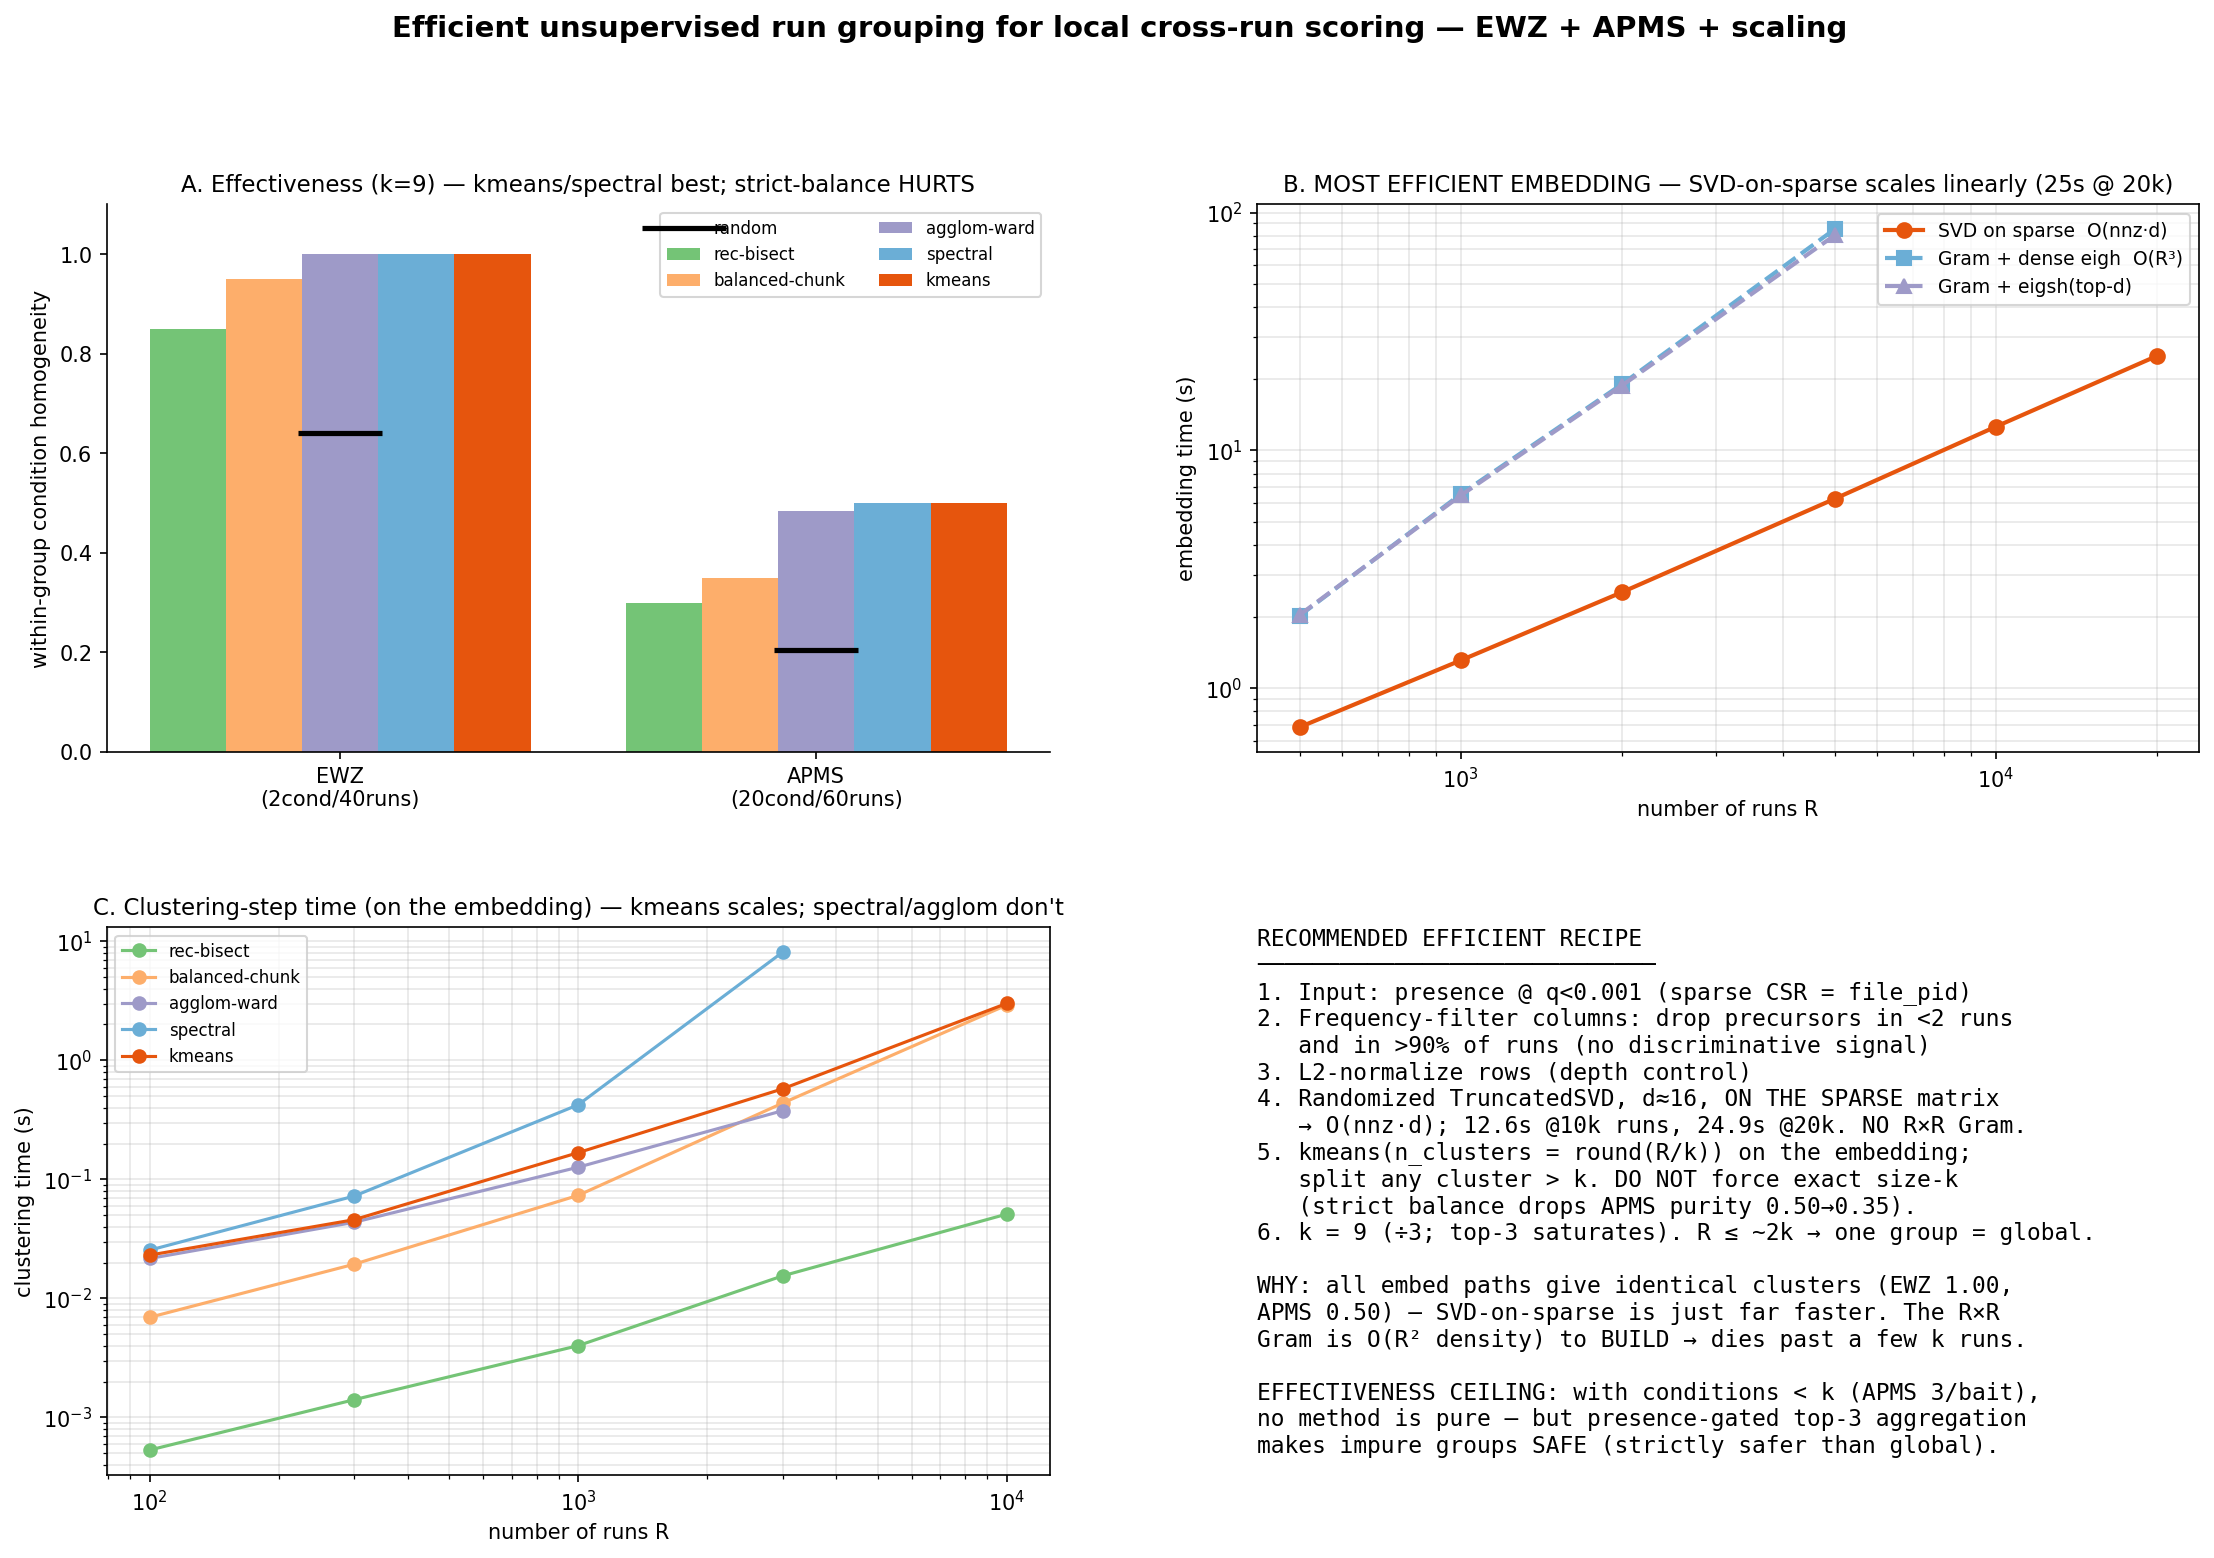
\includegraphics[width=\textwidth]{grouping_final.png}
\caption{Effectiveness (A), embedding scaling (B), clustering-step scaling (C), and the recommended
recipe (D). SVD-on-sparse is the linear-scaling embedding; k-means the scalable top method.}
\label{fig:final}
\end{figure}

\section{Finding 3: robustness --- only $k$ is a real knob}
Sweeping each hyperparameter one-at-a-time (Fig.~\ref{fig:robust}): EWZ stays at $1.00$ across
\emph{everything} (q-threshold $10^{-4}$--$10^{-2}$, SVD dim $4$--$48$, max-frequency $0.5$--$1.0$,
min-runs $2$--$10$, $k$ $6$--$15$); APMS is flat $\approx0.50$ across all but $k$. \textbf{The
defaults are safe --- they are not sensitive.} The one real dial is $k$, which trades purity against
breadth: on small-condition data (APMS, 3 runs/condition) homogeneity falls with $k$
($k{=}6\!:0.73$, $k{=}9\!:0.50$, $k{=}12\!:0.38$). Because the top-3 aggregation saturates at three
corroborators, small $k$ costs little breadth on small conditions but is purer; large $k$ fragments
large conditions less but mixes small ones more. \textbf{$k=9$ is a balanced default; $k=6$ if
false-transfer safety is paramount} (both divisible by 3).

\begin{figure}[h]\centering
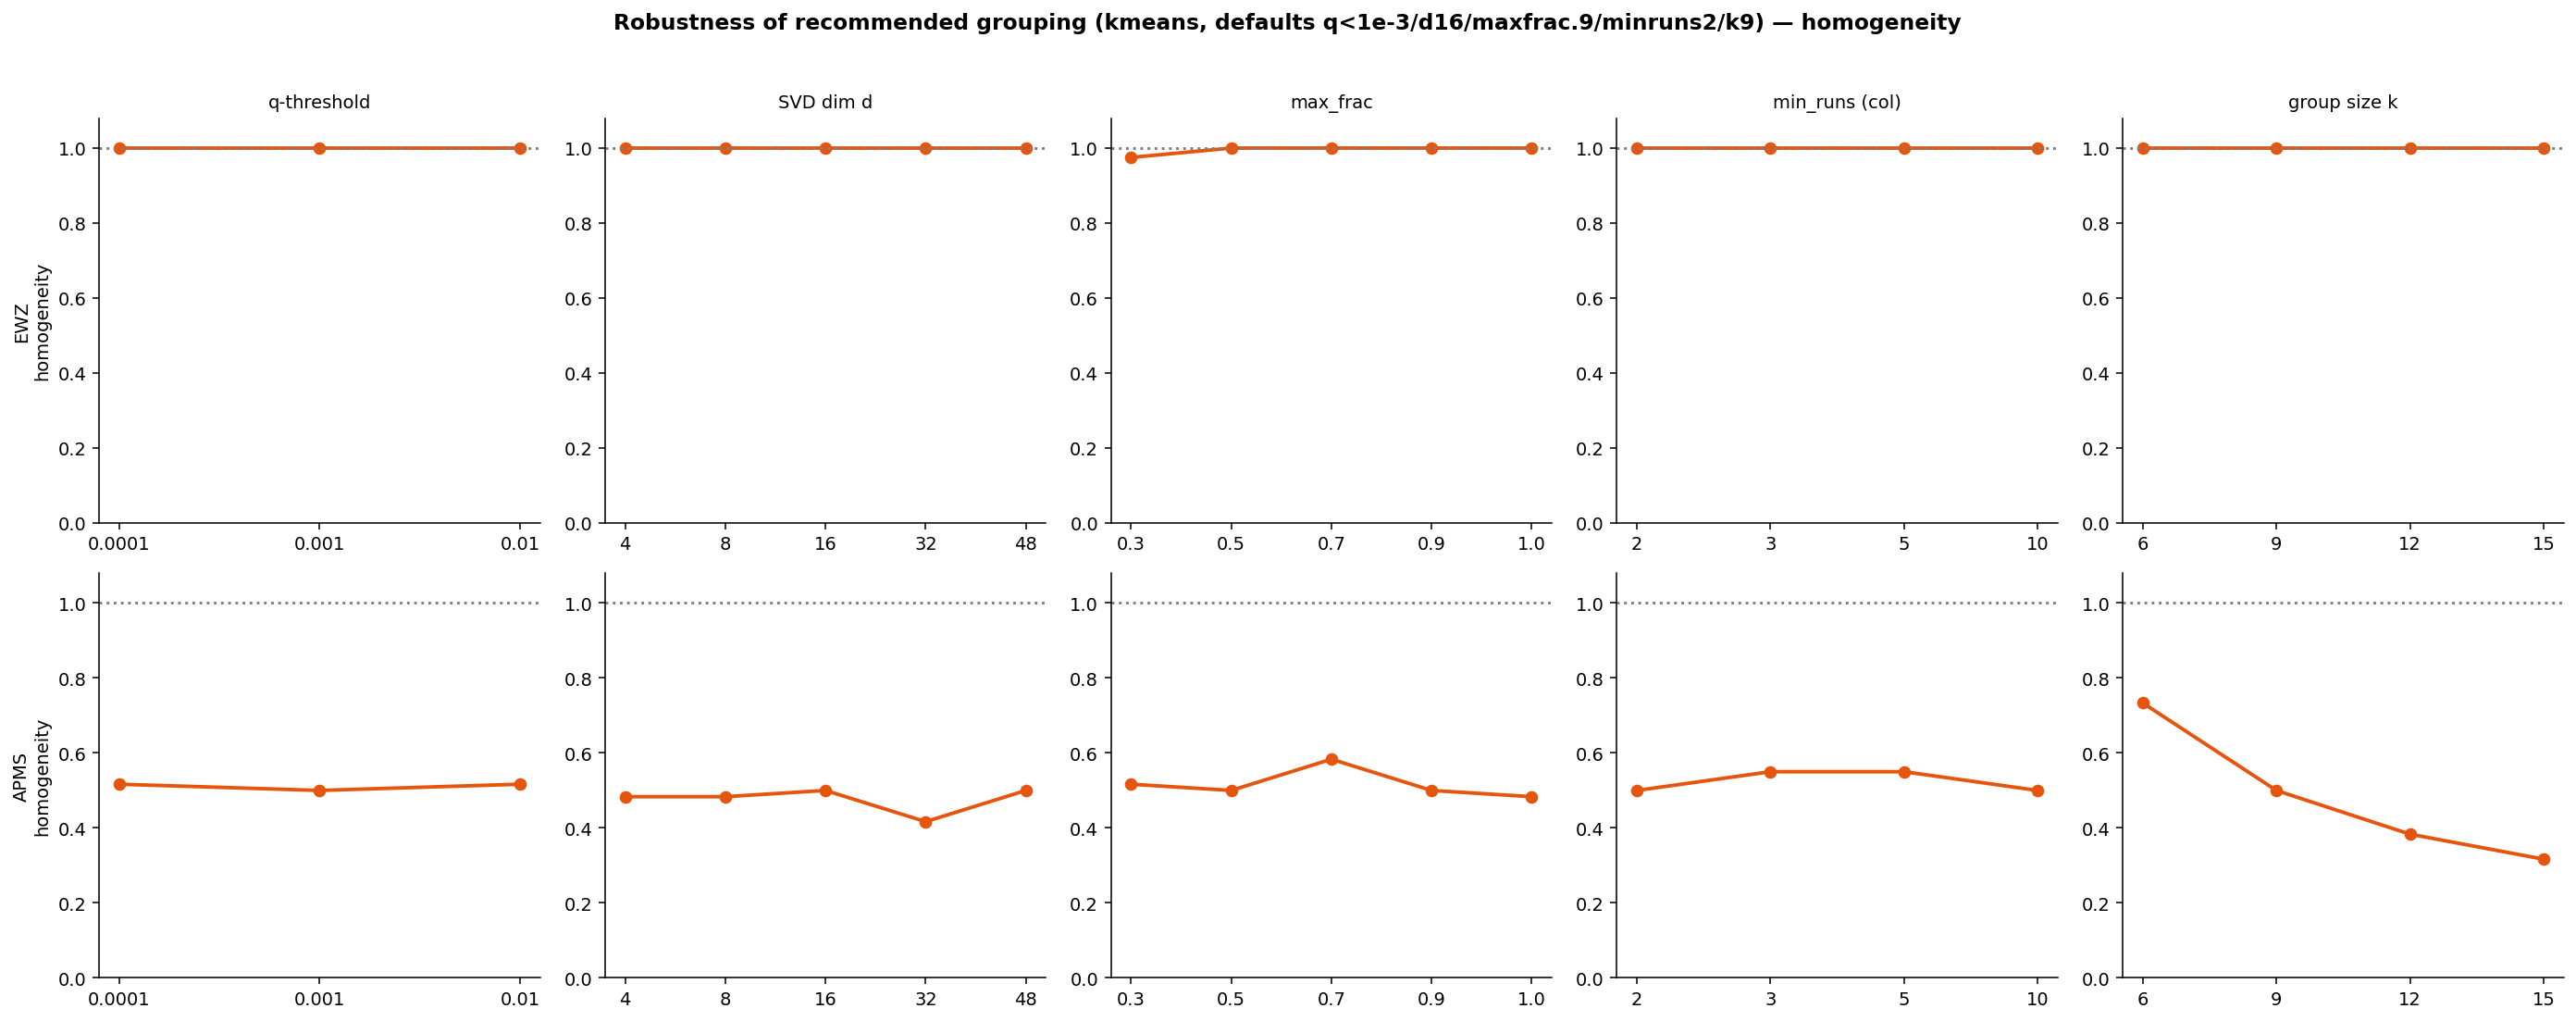
\includegraphics[width=\textwidth]{grouping_robustness.png}
\caption{Homogeneity vs.\ each hyperparameter (k-means, $k{=}9$). Only $k$ (rightmost) moves the
APMS result; all else is flat. EWZ is $1.00$ throughout.}
\label{fig:robust}
\end{figure}

\section{Finding 4: two design refinements}
\subsection{Minimum group size (instead of strict equal size)}
Rather than force equal size, floor small groups: merge any group below a minimum ($\sim$6--12) into
its nearest group by embedding centroid. This has an \textbf{honest tradeoff}:
\begin{itemize}[nosep]
  \item \textbf{EWZ:} beneficial --- small groups are \emph{fragments of a large (20-run) condition};
  merging them back keeps everything same-condition, homogeneity stays $1.00$. \code{min\_size}
  $1\!\to\!6\!\to\!9$: 7 $\to$ 5 $\to$ 2 groups, homogeneity $1.00$ throughout.
  \item \textbf{APMS:} \emph{harmful} --- small groups are already-pure 3-run bait triplets; merging
  them mixes baits without adding real corroborators (a bait-specific precursor's absent neighbours
  contribute $0$ to the top-3 anyway). \code{min\_size} $6$ drops homogeneity $0.50\!\to\!0.30$.
\end{itemize}
Interpretation: a minimum-size floor helps re-merge \emph{fragments of large conditions} but can
lower purity where small \emph{whole} conditions dominate. Since the presence-gated top-3 already
makes impure groups safe (absent members contribute $0$) and tiny \emph{pure} groups already hold
their true corroborators, a \textbf{modest floor ($\sim$6) with nearest-neighbour merge} is a
reasonable safeguard against corroborator-starved fragments; a large floor is not advised.

\subsection{Cluster separately per cross-validation fold}
The grouping is \emph{part of the feature computation}, so it must respect the same CV discipline as
the OOF $s_1$ it aggregates: build the run grouping \textbf{separately for each precursor-keyed CV
fold}, from that fold's own OOF presence. The two folds hold \emph{disjoint} precursor sets, so their
groupings are derived from independent evidence and \textbf{need not --- and generally will not ---
match}. That independence \emph{is the point}: a single shared grouping (derived from all precursors)
would leak one fold's information into the other fold's scoring. Divergence between the folds is
therefore expected and correct, not a defect.

Consequently the quality check is a \textbf{per-fold, within-fold} property --- each fold's grouping,
measured on its own, must be condition-coherent enough not to pool distinct conditions (the safety
invariant). Both folds pass independently:
\begin{center}\small
\begin{tabular}{lcc}
\toprule
dataset & per-fold homogeneity (each fold, measured alone) & (incidental) ARI(fold0, fold1) \\
\midrule
EWZ  & $1.00$ and $1.00$ & $0.684$ \\
APMS & $0.30$ and $0.30$ & $0.907$ \\
\bottomrule
\end{tabular}
\end{center}
The cross-fold ARI is \textbf{not a target and not required} --- a low value would be perfectly
acceptable, since we are not trying to reproduce a shared structure. It is reported only as an
incidental note on signal strength (here the condition signal happens to be strong enough that each
fold independently lands near the same structure; EWZ's $0.68$ merely reflects that the arbitrary
within-condition sub-split differs between folds, while both stay fully pure). Per-fold clustering is
the proper, OOF-consistent choice, and each fold's grouping is as good \emph{on its own} as the global
one.

\textbf{Isolation refinement.} For the fold isolation to be truly clean, the presence used to build
each fold's grouping should come from \emph{that fold's own OOF} $s_1$ (the same scores the feature
aggregates), not from a shared experiment-wide $q$ computed with a model that saw both folds. The
grouping, its presence input, and the aggregated scores are then all one fold's OOF product, end to
end.

\section{Recommended recipe}
\begin{enumerate}[nosep]
  \item \textbf{Per CV fold}, using only that fold's own OOF data (no cross-fold sharing):
  \item Presence at $q<10^{-3}$ from the fold's OOF $s_1$ (sparse CSR = \code{file\_pid}).
  \item Frequency-filter columns: drop precursors in $<2$ runs and in $>90\%$ of runs.
  \item $L_2$-normalize rows (depth control).
  \item Randomized \code{TruncatedSVD}, $d\approx16$, \textbf{on the sparse matrix} (no $R\times R$
  Gram) --- $O(\text{nnz}\cdot d)$, $\sim$13\,s at 10k runs.
  \item \code{k-means}$(n_{\text{clusters}}=\text{round}(R/k))$ on the embedding; \emph{split} any
  cluster $>k$; optionally \emph{merge} any group $<$ min-size ($\sim$6) into its nearest.
  \item $k=9$ (divisible by 3; top-3 saturates). When $R\le\sim2k$, one group $=$ all runs (recovers
  today's global behaviour, no code-path divergence).
\end{enumerate}
Total $\approx$30\,s at 20{,}000 runs; memory dominated by the sparse matrix. The feature is then
\code{group\_top3\_logodds}: the leave-one-out top-3 positive-logit sum within the run's group,
grafted onto the shadow decoys like \code{global\_max}. Effectiveness ceiling on
smaller-than-$k$ conditions is inherent, but the presence-gated aggregation makes impure groups safe
--- \textbf{grouping is strictly safer than the global feature regardless of purity}.

\end{document}
